\newpage
\section{Lecture 6:  Lax-Richtmyer analysis} 

Topics today: 
\begin{itemize}
    \item Lax-Richtmyer analysis of $D_t^+ u = D_x^+ D_x^- u$ in the 1-norm and 2-norm 
    \item Amplification factor  
\end{itemize}

\vspace{1em}
\hrule 
\vspace{1em} 

\subsection{Lax-Richtmyer Analysis for 1-norm} 
Recall that we can think of $B$ as an infinite tridaigonal Toeplitz matrix.  The max norm is the maximum absolute row sum: 
\[
    \|B\|_\infty = |\nu| + |1-2\nu| + |\nu| = \begin{cases}
        1, &\text{ if } 0\le \nu \le \frac{1}{2} ;\\
        4\nu -1, &\text{ if } \nu >\frac{1}{2} ;\\
        1-4\nu, &\text{ otherwise} .
    \end{cases}
\]
Note that the last case is not important since $\nu$ is always positive. Similary, $\|B\|_1$ is the maximal absolute column sum, which has the same value as $\|B\|_\infty$ in this case.  Hence, one can repeat the Lax-Richtmyer analysis for the 1-norm: 
\[
    \cB = L^1(\RR), \|g\|_1 = \int_{-\infty}^\infty |g(x)| \, dx. 
\]
Here $\cB_h = l_h^1$ is the summable sequences.  We have 
\[
    \|g\|_{1,h} = h \sum_{j=-\infty}^{\infty} |g_j|.  
\]
The $h$ in the norm definition doesn't affect the ``max absolute column sum'' formula for the $l^1$-norm since: 
\[
    \sum_{ u\neq 0 } \frac{\|Bu\|_{1,h}}{\|u\|_{ 1,h } } = \frac{h\|Bu\|_{ 1,1 } }{h\|u\|_{1,1}} = \frac{\|Bu\|_{1,1}}{\|u\|_{1,1}}.  
\]
Hence, one can still prove that 
\[
    \|\tau^n \|_{1,h} \le \begin{cases}
        \left( \frac{k}{2}+ \frac{h^2}{12}\right) M, &\text{ if } \nu \neq \frac{1}{6} ;\\
        \left( \frac{k^2}{6}+ \frac{h^4}{360} \right) M, &\text{ otherwise} .
    \end{cases}
\]
But in the 1-norm analysis: 
\[
    M = \sup_{0\le h\le 1, 0,\le x\le h} h \sum_{j} |g^{(\mu)} (x+jh)|.  
\]

For the 1-norm, we have the error $e_j^n = u_j^n - u(jh, nk)$ satisfies that 
\[
    e^{n+1} = B e^n - k \tau^n. 
\]
Hence, 
\[
    \|e^n\|_{1,h} \le K kn \max_{0\le l\le n-1} \|\tau^l\|_{1,h}. 
\]
We need $\nu\le \frac{1}{2}$, so that $\|B^k\|\le K =1$ and now we need $h\le 1$, or $k\le \epsilon = \nu$.  So that $\tau$ bound holds. Results: 
\[
    \sup_{0\le nk\le T} h \sum_{j=-\infty}^{\infty} |e_j^n| \le \begin{cases}
        \left( \frac{k}{2} + \frac{h^2}{12} \right)TM , &\text{ if } \nu \neq \frac{1}{6}, \nu \le \frac{1}{2} ;\\
        \left( \frac{k^2}{2} + \frac{h^4}{360} \right) TM, &\text{ otherwise } \nu = \frac{1}{6} .
    \end{cases} 
\]

\subsection{Amplification factor} 
As for the 2-norm,  we have 
\[
    \cB = l^2 (\RR), \quad \|g\| = \sqrt{\int_{-\infty}^{\infty} |g(x)|^2\, dx } 
\]
and 
\[
    \cB_h = l_h^2, \quad \|g\|_{2,h} = \sqrt{h \int_{j=-\infty}^{\infty} |g_j|^2 } 
\]
To determine the norm of $\|B^n\|_{2,h}$, we need to compute the amplification factor of $B$.  Given the finite difference operator: 
\[
    B u_j = \nu u_{j+1} + (1-2\nu) u_j + \nu u_{j-1}. 
\]
Then the amplification factor is: 
\[
    G(\xi) = \nu u e^{i\xi} + (1-2\nu) e^0 + \nu e^{-i\xi} = 1-4\nu \sin^2 \frac{\xi}{2}. 
\]
We will see that $\|B\|_{l_h^2} = \|G\|_\infty$.  Here we consider 
\[
    \|G\|_\infty = \max_{-\pi \le \xi \le \pi} |G(\xi)| = \max_{-\pi \le \xi \le \pi} \left| 1-4\nu \sin^2 \frac{\xi}{2} \right| . 
\]
%────────────────────────────────────────
\begin{figure}[H]
    \centering
    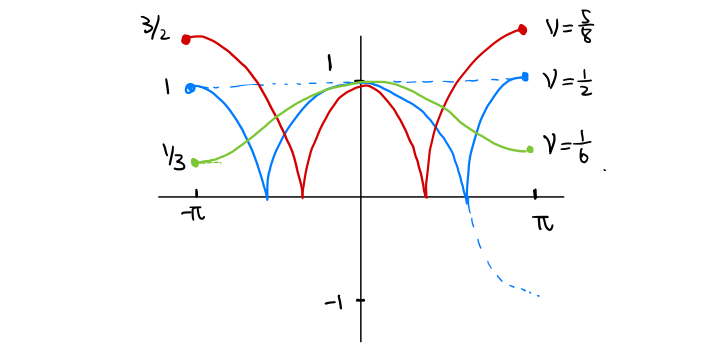
\includegraphics[width=0.6\textwidth]{figures/6-amplification.png}
\end{figure}
%────────────────────────────────────────
As expected, the transition from $\|B\| >1 $ to $ \|B\|\le 1 $ occurs at $\nu = \frac{1}{2}$.  The rest of the Lax-Richtmyer convergence proof in the 2-norm is very similar to the 1-norm analysis. First we will show that 
\[
    \|\tau^n \|_{2,h} \le \begin{cases}
        M \sqrt{\frac{2}{3}k^2 + \frac{1}{63}h^4} , &\text{ if } \nu \neq \frac{1}{6} ;\\
        M\sqrt{\frac{k^4}{10}+\frac{h^8}{39600}} , &\text{ otherwise} .
    \end{cases}
\]
Here $M = \max_{0\le h\le 1, 0\le x \le h} \sqrt{h \sum_j |g^{(\mu)} (x+jh)|^2}$.  Conclusion for Lax-Richtmyer: if $\nu\le \frac{1}{2}$ and $0\le k\le v$ then $\|B(k)^n\|\le 1$ and 
\[
    \max_{0\le nk \le T} \sqrt{h\sum |e_j^n|^2} \le \begin{cases}
        MT\sqrt{\frac{2}{3}k^2 + \frac{1}{63}h^4} , &\text{ if } \nu \neq \frac{1}{6}, \nu\le \frac{1}{2} ;\\
        MT\sqrt{\frac{k^4}{10} + \frac{h^8}{39600}} , &\text{ otherwise} .
    \end{cases}
\]


%────────────────────────────────────────
\begin{note}
The 2-norm analysis (Von-Neumann stability analysis) is the version that generalizes most easily to implicit methods. 
\end{note}
%────────────────────────────────────────
